%%% Demographic Research Pandoc Style
%%% Jonas Schöley
%%% 2019-01-25
%%% Depends on file "DemRes.bst" for custom bibliography styling.

\documentclass[10pt, twoside, parskip=half]{article}
\raggedbottom

%%%% font/encoding %%%%%%%%%%%%%%%%%%%%%%%%%%%%%%%%%%%%%%%%%%%%%%%%%%%%%%%%%%%%

\usepackage[utf8]{inputenc}          % .tex-file text encoding
\usepackage[T1]{fontenc}             % vector fonts and special chars in output
\usepackage{times}                   % Times Roman font family

%%%% maths %%%%%%%%%%%%%%%%%%%%%%%%%%%%%%%%%%%%%%%%%%%%%%%%%%%%%%%%%%%%%%%%%%%%

\usepackage{mathrsfs} % maths script fonts
\usepackage{amssymb}  % maths symbols
\usepackage{amsmath}  % various maths features

%%%% figures %%%%%%%%%%%%%%%%%%%%%%%%%%%%%%%%%%%%%%%%%%%%%%%%%%%%%%%%%%%%%%%%%%


\usepackage{graphicx}

%%%% captions %%%%%%%%%%%%%%%%%%%%%%%%%%%%%%%%%%%%%%%%%%%%%%%%%%%%%%%%%%%%%%%%%

\usepackage{float}      % captions above
\usepackage[hang]{caption}
\DeclareCaptionLabelSeparator{capsep}{:\hspace{1cm}}
\captionsetup[figure]{
            labelsep        = capsep,
            name            = Figure,
            font            = bf,
            labelfont       = bf,
            justification   = raggedright,
            singlelinecheck = false
}

\captionsetup[table]{
            labelsep        = capsep,
            name            = Table,
            font            = bf,
            labelfont       = bf,
            justification   = raggedright,
            singlelinecheck = false
}

% captions above
\floatstyle{plaintop}
\restylefloat{table}
\restylefloat{figure}

%%%% localization %%%%%%%%%%%%%%%%%%%%%%%%%%%%%%%%%%%%%%%%%%%%%%%%%%%%%%%%%%%%%

% babel
\usepackage[english]{babel}         % document language/localization
\usepackage[htt]{hyphenat}          % hyphenation rules

%%%% bibliography %%%%%%%%%%%%%%%%%%%%%%%%%%%%%%%%%%%%%%%%%%%%%%%%%%%%%%%%%%%%%

\usepackage{natbib}
\setcitestyle{aysep={}}
\bibliographystyle{DemRes}
\newcommand{\doi}[1]{\href{http://www.dx.doi.org/#1}{\textcolor{blue}{doi:#1}}}

%%%% layout %%%%%%%%%%%%%%%%%%%%%%%%%%%%%%%%%%%%%%%%%%%%%%%%%%%%%%%%%%%%%%%%%%%

\usepackage{geometry}
\geometry{
  paperheight = 22cm,
  paperwidth  = 17cm,
  top         = 2.54cm,
  bottom      = 2.54cm,
  inner       = 2cm,
  outer       = 2.54cm,
  footskip    = 11mm,
  headheight  = 1cm,
  headsep     = 0.75cm,
  showframe   = false
}

% change spacing
\setlength{\parskip}{0ex}
\setlength{\parindent}{.7cm}
\setlength{\bibsep}{.18cm}

% no page numbers
\pagenumbering{gobble}

% avoid orphans and widows
\widowpenalty = 10000
\clubpenalty  = 10000

% don't break footnotes
\interfootnotelinepenalty = 10000

% don't hyphenate across pages
\brokenpenalty10000\relax

% tight lists
\providecommand{\tightlist}{%
  \setlength{\itemsep}{0pt}\setlength{\parskip}{0pt}}

%%%% sections %%%%%%%%%%%%%%%%%%%%%%%%%%%%%%%%%%%%%%%%%%%%%%%%%%%%%%%%%%%%%%%%%

% spacing
\makeatletter
\renewcommand\section{\@startsection {section}{1}{\z@}%
                                   {-24pt}%
                                   {2.3ex \@plus.2ex}%
                                   {\normalfont\large\bfseries}}
\renewcommand\subsection{\@startsection{subsection}{2}{\z@}%
                                     {-24pt}%
                                     {1.5ex \@plus .2ex}%
                                     {\normalfont\normalsize\bfseries}}
\makeatother

% style
\usepackage{titlesec}
\titleformat{\section}[hang]{\raggedright\normalfont\bfseries\large}{\arabic{section}.}{1ex}{}
\titleformat{\subsection}[hang]{\raggedright\normalfont\bfseries}{\arabic{section}.\arabic{subsection}}{1ex}{}
\titleformat{\subsubsection}[hang]{\raggedright\normalfont\bfseries}{\arabic{section}.\arabic{subsection}.\arabic{subsubsection}}{1ex}{}

%%%%% footnotes %%%%%%%%%%%%%%%%%%%%%%%%%%%%%%%%%%%%%%%%%%%%%%%%%%%%%%%%%%%%%%%

% Footnotes
\usepackage[bottom]{footmisc}
\setlength{\footnotemargin}{0.6em}

% if you have code in your footnotes, the million macro march
% kind of bumps into itself.
% Pandoc, having just rendered your text into LaTeX,
% knows whether the 'variable' `verbatim-in-note` is True, and
% If it is, it asks for a  LaTeX package that solves the dilemma:

%%%% tables %%%%%%%%%%%%%%%%%%%%%%%%%%%%%%%%%%%%%%%%%%%%%%%%%%%%%%%%%%%%%%%%%%%

  \usepackage{array,longtable,booktabs,multirow}
  % -- This is needed because raggedright in table elements redefines \\:
  \newcommand{\PreserveBackslash}[1]{\let\temp=\\#1\let\\=\temp}
  \let\PBS=\PreserveBackslash
  \usepackage{etoolbox} % global table format
  \AtBeginEnvironment{tabular}{\scriptsize\sffamily}

%%%% subscripts %%%%%%%%%%%%%%%%%%%%%%%%%%%%%%%%%%%%%%%%%%%%%%%%%%%%%%%%%%%%%%%


%%%% links %%%%%%%%%%%%%%%%%%%%%%%%%%%%%%%%%%%%%%%%%%%%%%%%%%%%%%%%%%%%%%%%%%%%

\usepackage{hyperref}
\hypersetup{
  hidelinks,
  breaklinks=true,
  pdftitle={Lexis Fields}
}

%%%% misc %%%%%%%%%%%%%%%%%%%%%%%%%%%%%%%%%%%%%%%%%%%%%%%%%%%%%%%%%%%%%%%%%%%%%

% for colored links
\usepackage{xcolor}

% Footnotes:

% For shaded code blocks

%%%% includes %%%%%%%%%%%%%%%%%%%%%%%%%%%%%%%%%%%%%%%%%%%%%%%%%%%%%%%%%%%%%%%%%

% header_includes
  \usepackage{placeins}

%%%% title, authors %%%%%%%%%%%%%%%%%%%%%%%%%%%%%%%%%%%%%%%%%%%%%%%%%%%%%%%%%%%

  \title{\large\textbf{Lexis Fields}\vskip 0em}
  \author{\normalsize\textrm{\textbf{(authors redacted)}}}
\date{\vspace{-5ex}}

%%%% document %%%%%%%%%%%%%%%%%%%%%%%%%%%%%%%%%%%%%%%%%%%%%%%%%%%%%%%%%%%%%%%%%

\begin{document}

  \maketitle

\vspace*{-24pt}
\vspace*{5mm}
\setlength{\parskip}{0.5em}
\section*{Abstract}
  \noindent\textbf{BACKGROUND}\\
  Lexis surfaces are an established visualization technique to show how a given value changes over age and time. Vector fields are a two-dimensional representation of two variables: direction and speed (or force).
  \par
  \noindent\textbf{OBJECTIVE}\\
  We aim to increase the dimensionality of patterns shown on the Lexis surface by placing a vector field on the Lexis surface.
  \par
  \noindent\textbf{RESULTS}\\
  We show Lexis fields of the relationship between life expectancy and the standard deviation of remaining lifespan over age and time. These instruments enable information layering on standard Lexis surfaces that is not common practice.
  \par
  \noindent\textbf{CONCLUSIONS}\\
  Lexis fields extend the descriptive and analytic power of the Lexis surface, and these can be designed to display information at higher densities than commonly made Lexis surfaces.
  \par
\vspace*{12pt}

\setlength{\parskip}{0ex}

\newpage

TODO TR: add area examples.

\hypertarget{introduction}{%
\section{Introduction}\label{introduction}}

Lexis surfaces are a graphical tool used to display data on the Lexis coordinate plane, a Cartesian plane that is also a simplex relationship between age, period, and cohort. Surfaces are often displayed as heat maps, contour maps, perspective plots, or variants of these things \citep{vaupel1987thousands}. Various kinds of quantities, such as raw magnitudes, differences \citep{minton2017visualising}, excesses \citep[\citet{acosta2019apc}]{remund2018cause} ratios \citep{canudas2005age}, intensities, proportions, derivatives \citep{rau2017visualizing}, and even compositions \citep{scholey2017visualizing} can be displayed on Lexis surfaces in order to put age, period, cohort, or other patterns in relief.

Vector fields are a graphical form generally used to display variation in speed, direction, or force over a plane \citep{weiskopf2007vector}. Point estimates of these quantities on the plane are often represented with segments or arrows, where length may be proportional to a function of magnitude (force, speed), and angle indicates direction, potentially disambiguated with an arrowhead or articulated as a curve.

Maps in general combine layers of categorical, continuous, and symbolic information on a common spatial projection. Lexis surfaces in contrast almost exclusively display one visual layer at a time. We propose to enrich Lexis surfaces by adding a visual layer of quantitative information coded symbolically as a vector field, and we liken this to cartographic information layering. We propose a fusion of Lexis surfaces and vector fields, \emph{Lexis fields}, as a tool to display variation in relationships between variables over age and time. A Lexis field may either be shown atop on a Lexis surface, representing two map layers --- a true Lexis map --- or as a single-layer stand-alone visualization. Visual patterns in a Lexis field reveal changes in complex relationships over age and time.

We give an overview of constructing a Lexis field with an application. Our example explores the relationship between remaining life expectancy and the standard deviation of remaining lifespan over age and time based on all available populations in the \citet{HMD} from 1950 onward. This example and others discussed motivate how Lexis fields could be used in other areas demographic research.

\hypertarget{lexis-field-construction}{%
\section{Lexis field construction}\label{lexis-field-construction}}

It makes sense to plot a Lexis field if data contain a relationship that can be summarized with a line, a simple curve, or similar, that varies by age and/or time. Constructing a Lexis field involves several design choices, which can however be codified into four basic steps, which we summarize in Fig. \ref{fig:one}. The steps to do so are outlined in the following description, referenced to regions of Fig. \ref{fig:one}.

\begin{quote}
\textbf{A} Determine a grid over age and time on which to condition data selection. For example, a five-year grid implies \(5\times 5\) Lexis cells. Data may be selected from multiple populations on the same reference grid or may consist in a selection of attributes from a single underlying Lexis surface. Presumably two variables are required.
\end{quote}

\begin{quote}
\textbf{B} Abstract a model from the data, such as a linear, parabolic, or similarly simple relationship.
\end{quote}

\begin{quote}
\textbf{C} Translate the model to the characteristics of a line segment, which we refer to as a field \emph{pointer}. For example, the pointer angle can relate to the model relationship, and length and color may be determined by other aspects of the model, such as \(r^2\) or the Pearson's correlation coefficient.
\end{quote}

\begin{quote}
\textbf{D} Draw the segment in the corresponding Lexis grid cell, repeating all steps for each cell in the diagram.
\end{quote}



\begin{figure}[!t]
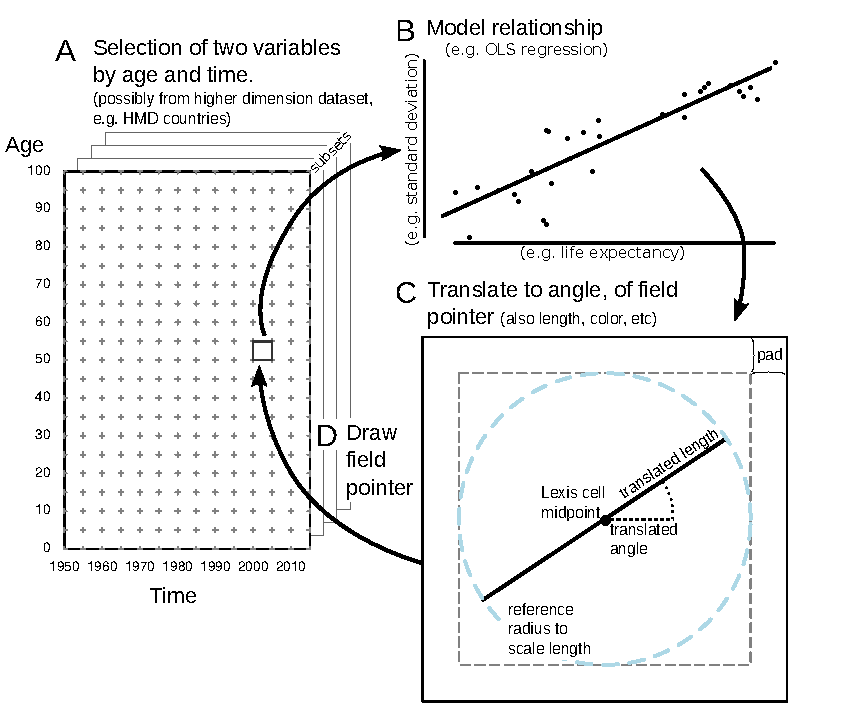
\includegraphics[width=1\linewidth]{Figures/ExplainerDiagram} \caption{A diagram depicting the translation of functional relationships in data conditioned on age and time to visual encoding on a Lexis field. \textbf{A}: Condition data selection on age and time. \textbf{B}: Fit a model (e.g.~linear) to the data subset. \textbf{C}: Translate the model to field elements, `pointers', using angle, and possibly also length, curvature, thickness, etc. to represent model qualities. \textbf{D}: Populate the Lexis plane with field pointers to create a Lexis field.}\label{fig:one}
\end{figure}
\FloatBarrier

\hypertarget{application}{%
\section{Application}\label{application}}

We select all HMD data available for females after 1950. For each life table we calculate an extra column for the standard deviation of remaining lifespan \(sd(x)\). Each Lexis field element is based on the relationship between \(sd(x)\) and remaining life expectancy \(e(x)\) in \(1\times 5\) Lexis cells \footnote{Data points included in regressions are single ages evenly divisible by five for each of the five years included in a Lexis reference cell.}, as summarized by bivariate linear regression over the data points in each cell. The regression results used for each Lexis cell in resulting Lexis fields are identical, but the translation of regressions to field pointers varies between designs. We offer four examples of Lexis field designs, each drawn on \(5\times 5\) Lexis subplots.

The first of these, Fig. \ref{fig:two}, is a bare-bones Lexis field that serves to illustrate the underlying concept. This display draws each regression slope as a line segment of equal length (4 ``years'' long) and centered on each Lexis cell. The slope of each pointer is identical to regression slopes, which may be justified in this case because \(e(x)\) and \(sd(x)\) are both in year units. This is the truest and most literal depiction of how these regression slopes vary over age and time among females. From this figure we can see, for example, that there is some age where the relationship turns from negative to positive, which increased slightly over time. Slopes dampened in younger ages around the 1980s, but have since increased (except infants).



\begin{figure}[!t]

{\centering 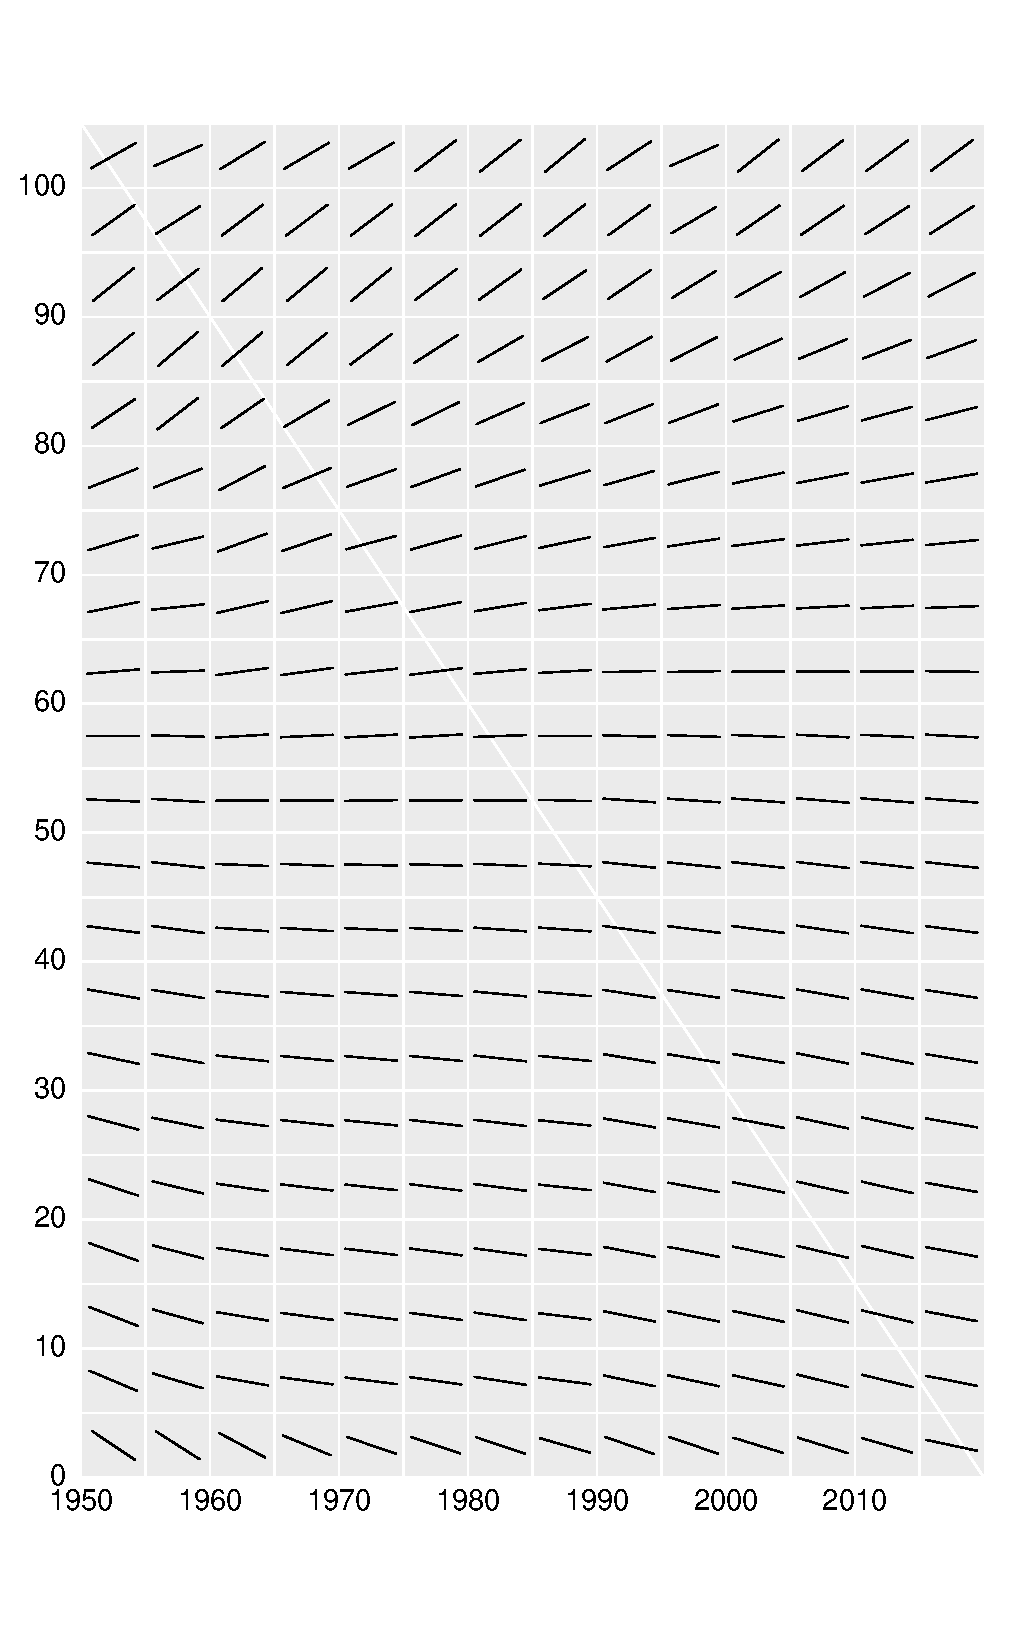
\includegraphics[width=0.8\linewidth]{Figures/FigApp1} 

}

\caption{Lexis field: \(sd(x)\) by \(e(x)\) linear fits, with slopes drawn equal to regression line slope coefficients. Pointer lengths are all equal.}\label{fig:two}
\end{figure}

The second version, Fig. \ref{fig:three}, draws the same slopes multiplied by two, with pointer lengths scaled proportional to the between-population interquartile range of the \(e(x)\) and \(sd(x)\) values used in regressions\footnote{Specifically, pointer length is proportional to the central spread of the relationship between \(e(x)\) and \(sd(x)\), approximated as \(\sqrt{IQR(e(x))^2 + IQR(sd(x))^2}\)}, and line weight and grayscale proportional to the \(r^2\) of the regression fit. Segment lengths are therefore indicative of the spread in the data, while higher \(r^2\) results in darker and thicker pointers.



\begin{figure}[!t]

{\centering 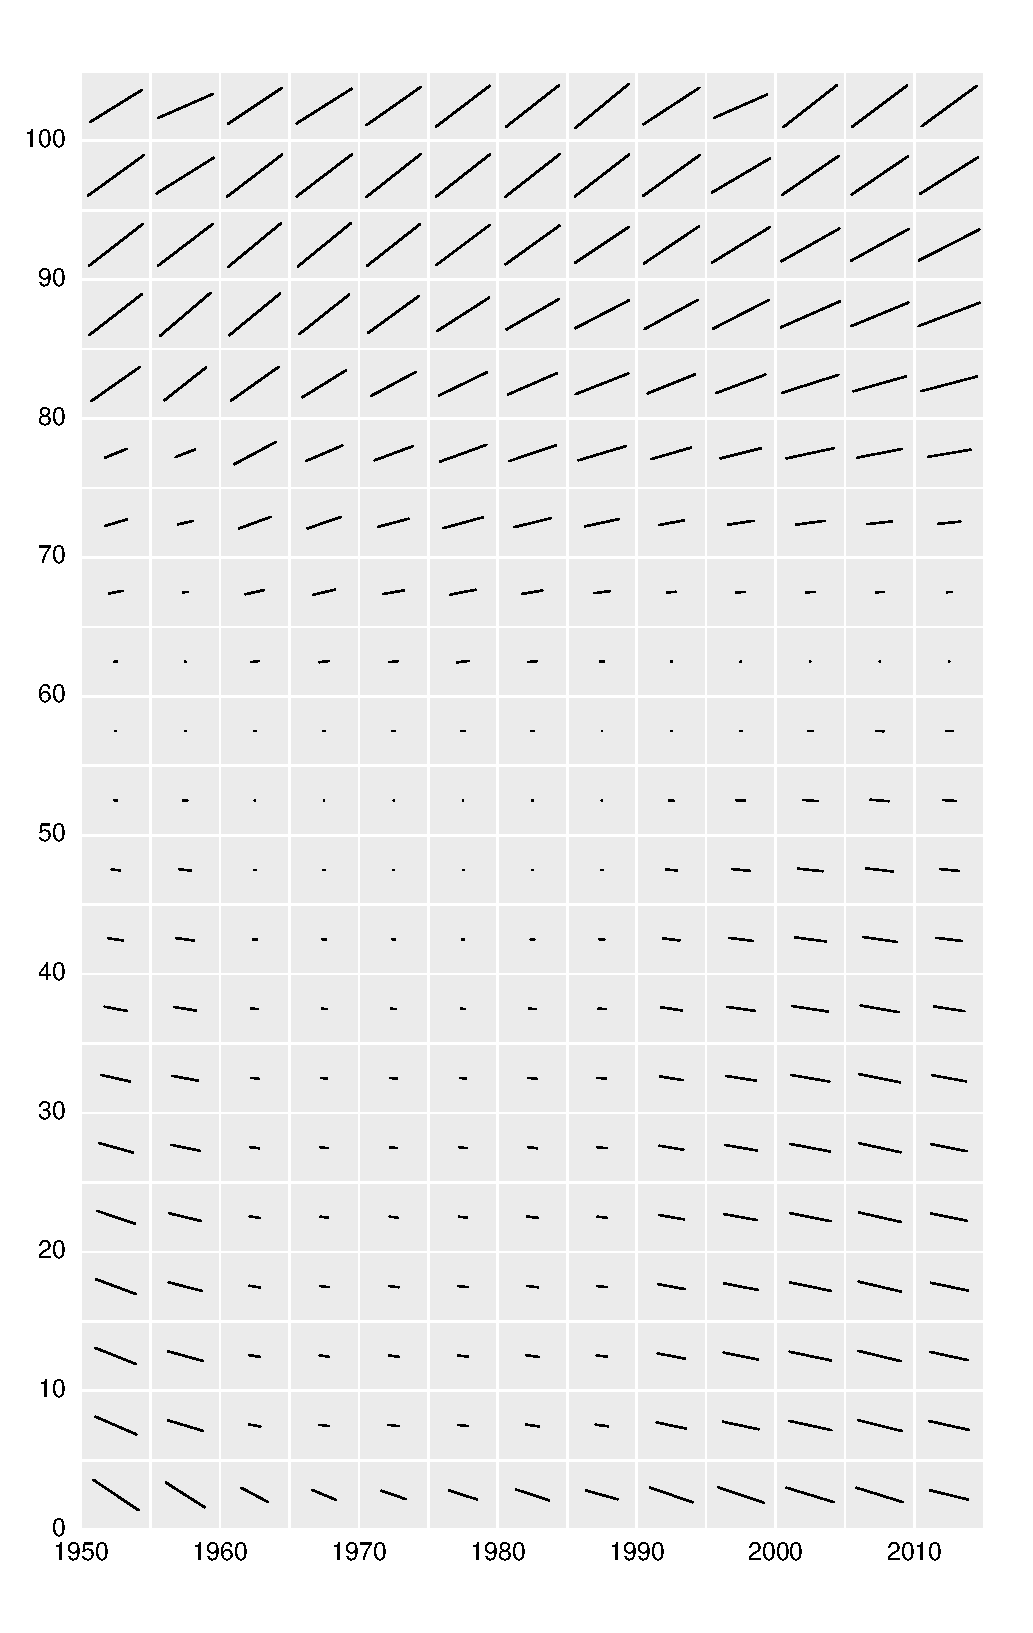
\includegraphics[width=0.8\linewidth]{Figures/FigApp2} 

}

\caption{Lexis field: \(sd(x)\) by \(e(x)\) linear fits, with slopes exaggerated by 2. Pointer length is proportional to the diagonal of the IQR box around \(sd(x)\) and \(e(x)\), while grayscale and segment width are proportional to \(r^2\) (darker and thicker = higher \(r^2\)).}\label{fig:three}
\end{figure}

The final example, Fig. \ref{fig:four} is a true Lexis map. The base of the map is a filled contour plot of the mean (over HMD populations) of the lifetable survivorship column \(\ell(x)\), converted to proportions. This quantity is interpreted as the probability of surviving from birth until at least age \(x\), which means that contours in the Lexis map are interpreted as survivorship quantiles. The survivorship surface is redundantly drawn with a sequential color palette and labelled contours. The same field from Fig. \ref{fig:four} is layered atop the survivorship quantile surface, achieving a true layered map.



\begin{figure}[!t]

{\centering 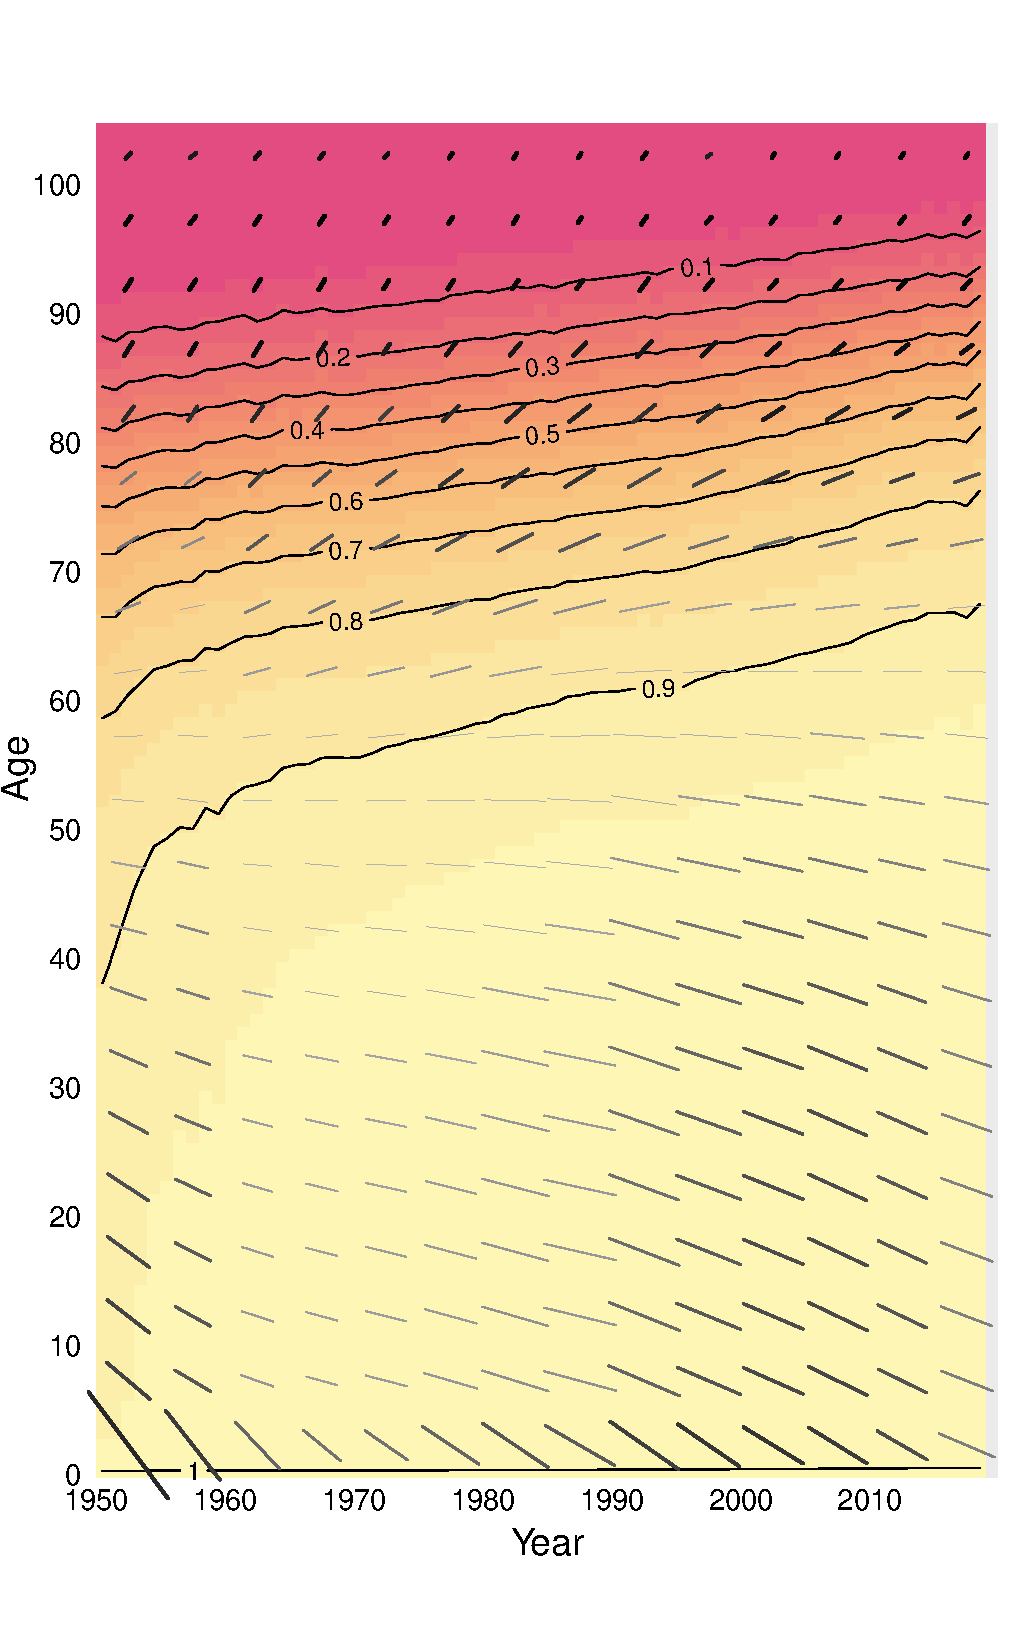
\includegraphics[width=0.8\linewidth]{Figures/FigApp3} 

}

\caption{A Lexis map: Lexis surface of mean survivorship quantiles as a filled contour plot plus a Lexis field of \(sd(x)\) by \(e(x)\) linear fits, slopes exaggerated by 2. Pointer length is proportional to the diagonal of the IQR box around \(sd(x)\) and \(e(x)\), while grayscale and segment width are proportional to \(r^2\).}\label{fig:four}
\end{figure}
\FloatBarrier

\hypertarget{discussion}{%
\section{Discussion}\label{discussion}}

We suggest the use of vector fields on the Lexis surface, introducing the notion of a Lexis field, which is a standard vector field on a regular Lexis grid over age and time. This instrument allows researchers to overlay Lexis surfaces and display relationships in complex ways. We demonstrate some of the designer freedom in translating data into the elements of a Lexis field, as well as an instance of Lexis map layering. These examples serve to illustrate the construction of Lexis fields, but do not pretend to be \emph{best practice} Lexis surfaces in terms of visual design or legibility. It is our sense that the patterns revealed in Figures \ref{fig:two}-\ref{fig:four} are accessible to the viewer and lend themselves to substantive interpretation. The field pointers we use represent linear models. Although patterns in data may be much more complex than can be expressed with a single linear model, in fields each model fit can be thought of as a local \emph{zoom-in} on a complex macro pattern --- subtle changes between neighboring pointers reveal interpretable patterns as the eye \emph{zooms out}.

The composite surfaces of \citet{scholey2017visualizing} also display layered information as a single visual layer. Small multiples of Lexis surfaces (for example panel plots of Lexis surfaces) on the other hand constitute a de-layering \citep[c.f.][\citet{kashnitsky2019geofaceting}]{remund2018cause}, as these are spatially disjoint. Comparisons between plots require an extra attentive step from the the viewer to cross-reference patterns or values at specific coordinates of age and time. More dimensions (e.g.~causes of death) imply more such cross-referencing work from the viewer if displayed in this way. On the other hand, an overlaid Lexis field may imply a lower degree of age and time resolution for each of the variables overlaid --- for example we used a \(5\times 5\) grid in our application. We do not evaluate the trade-off between the potential clarity of individual but disjoint graphs versus comparisons using Lexis fields. Researchers may wish to experiment using the reproducible code we provide.

The idea to draw a Lexis field arose in practice in an attempt to investigate the apparently mechanical relationship between lifespan variation and average length of life with a macro view. Evidence suggests a negative relationship between lifespan variation and life expectancy when measured at young ages such as 0 or 15 \citep[\citet{smits2009length},\citet{vaupel2011life},\citet{alvarez2019latin},\citet{colchero2016emergence}]{wilmoth1999rectangularization}. This means that at the aggregate level, as life expectancy at birth increases in low mortality countries, length of life becomes more equal, and this relationship appears to hold up generally between human populations \citep{colchero2016emergence}. Lifespan variation has become an important topic in demographic research because larger lifespan variation implies greater uncertainty about the timing of death for individuals and, at the population level, it implies that health improvements are unevenly shared in a population \citep{van2018case}. More recently, several cases have been uncovered where an increase in life expectancy is not followed by decrease in lifespan variation. For example, in Eastern Europe, in periods of slow improvements in life expectancy at birth, lifespan variation moved in the same direction, running against the usual narrative \citep{aburto2018lifespan}. Similarly, studies have pointed out that the age used for truncation is important to determine the strength and direction of the relationship between life expectancy and lifespan variation \citep[\citet{nusselder1996rectangularization}, \citet{robine2001redefining}, \citet{engelman2010implications}, \citet{nemeth2017life}]{myers1984compression}.
Our visual approach reveals that the relationship starts as strongly negative, and somewhere near age 55 it reverses to become positive in a systematic way. A crossover was already documented by \citet{myers1984compression}, but it has not been previously shown in such a systematic and comprehensive way, possibly because standard ways of looking at these data would have required dozens or hundreds of graphs. We aim to fill this gap by proposing a way to visualize these complex patterns in a single plot.

Fig.\ref{fig:four} serves to illustrate that Lexis fields can be layered with traditional Lexis surfaces that are color-coded, increasing the information and pattern density on the Lexis plane with little drawback in terms of legibility. This allows the viewer to interpret field patterns conditional on the underlying surface. For example, the increase in the (mean) 90\% survival contour appears to have been faster than the increase in the age at which pointer slopes switch from negative to positive. Few people reach ages in which there is a strong positive relationship between lifespan uncertainty and average remaining lifespan, but the fraction who do so is increasing.

Fields could also be derived from a single underlying pattern rather than a series of regressions on different populations or variables. For example, \citet{shang2018visualizing} recommends the use of phase diagrams to represent the rate of change of the hypothetical life course implied by period fertility curves. This construct could be translated to a Lexis field in a straightforward way, with pointers mapping to the notions of acceleration and velocity. Certainly variants of vector fields could be used to intuitively display other demographic phenomena and components of demographic change, and these do not need to adhere to the Lexis grid. For example, changes in the relationship between male and female fertility rates over age and time could be shown with a field. Other well-known relationships, such as the \emph{Preston curve} \citep{preston1975changing} or \emph{Taylor's Law} \citep{cohen2018gompertz}, might also lend themselves to Lexis field representation. We also suggest wider use of fields based on demographic relationships in spatial settings.

\hypertarget{conclusions}{%
\section{Conclusions}\label{conclusions}}

We describe the construction and use of vector fields on the Lexis plane. We argue that this technique can increase the information density and scope displayed on the Lexis surface. We also argue that fields are easily made compatible with Lexis surfaces drawn as filled contour plots, which lends them to map layering. We suggest alternative field designs and uses that could be easily applied for other demographic processes and research questions. In sum, displaying a larger variety of demographic quantities on the Lexis plane and increasing the information density on the Lexis plane using layering techniques such as fields should broaden the scope of demographic exploration and sharpen the instruments of demographic pattern detection.

\hypertarget{reproducibility}{%
\section{Reproducibility}\label{reproducibility}}

Calculations and visualizations in this manuscript were all done in the R programming language \citep{R}. Code used to produce the experimental visualizations here is available in a public repository:

\url{https://github.com/timriffe/MacroShape/DR}

\hypertarget{acknowledgements}{%
\section{Acknowledgements}\label{acknowledgements}}

We wish to thank Alyson van Raalte for helpful comments received that improved this manuscript.

\clearpage

\newpage

\bibliography{references.bib}

\end{document}
